\documentclass{article}
\usepackage{tikz}
\usetikzlibrary{cd}
\usepackage[utf8]{inputenc}
\usepackage[english]{babel}
\usepackage{amsfonts}
\usepackage{amsthm}
\usepackage{amsmath}
\usepackage{amssymb}

\newtheorem{theorem}{Theorem}
\newtheorem{es}{Examples}

\newcommand{\inter}[1]{int(#1)}

\title{MATC27 Assignment 4}
\author{Anmol Bhullar - 1002678140}

\begin{document}
    \maketitle
    \textbf{P1.}\\ 
    In order to show $d_U$ is a metric on $U$, we have to that for all $x,y,z\in U$ the following conditions hold: (i) $d_U(x,y)\geq 0$ (ii) $d_U(x,y)=0
    \leftrightarrow x=y$ (iii) $d_U(x,y)=d_U(y,x)$ and (iv) $d_U(x,z)\leq d_U(x,y)+d_U(y,z)$\\
    (i) It is clear that $|\frac{1}{d(x,U^c)} - \frac{1}{d(y,U^c)}|\geq 0$ (property of the absolute sign). Furthermore, since $U\subseteq X$, we have that
    $x,y\in X$ and since $d$ is a metric on $X$, we know $d(x,y)\geq 0$.
    Thus, it follows that $0 + 0 \leq d(x,y) + |\frac{1}{d(x,U^c)}-\frac{1}{d(y,U^c)}| = d_U(x,y)$
    so that $d_U(x,y)\geq 0$ as wanted.


    (ii) Assume $x=y$, we show $d_U(x,y)=0$. Note, since $x,y\in X$, we have $d(x,y)=0$ since $d$ is a metric space. 
    Furthermore, 
    \[ |\frac{1}{d(x,U^c)}-\frac{1}{d(y,U^c)}| =  |\frac{1}{d(x,U^c)} - \frac{1}{d((x),U^c)}| = |0| = 0\] 
    so that $d_U(x,y) = d(x,y) + |\frac{1}{d(x,U^c)} - \frac{1}{d(y,U^c)}| = 0 + 0 = 0$ as wanted.
    Now, assume $d_U(x,y)=0$, we show $x=y$.  Consider:
    \begin{align*}
        0 = d_U(x,y) = d(x,y) + |\frac{1}{d(x,U^c)} - \frac{1}{d(y,U^c)}| \\
        \implies d(x,y) = -|\frac{1}{d(x,U^c)} - \frac{1}{d(y,U^c)}|
    \end{align*}
    Since $d$ is a metric, we know $d(x,y)\geq 0$ and because of the absolute value signs, we know the right hand side (w/out the $-1$ factor) must also be
    $\geq 0$. Therefore, $d(x,y) = 0 = |\frac{1}{d(x,U^c)} - \frac{1}{d(y,U^c)}|$.
    Again since $d$ is a metric, we know that $d(x,y) = 0$ if and only if $x=y$. Thus, $d_U(x,y) = 0 \implies x=y$ as wanted.


    (iii) Note $d(x,y) = d(y,x)$ since $d$ is a metric space. Also, since $|a-b| = |b-a|$ for all real numbers $a$ and $b$, we obtain the fact:
    \[|\frac{1}{d(x,U^c)} - \frac{1}{d(y,U^c)}| = |\frac{1}{d(y,U^c)} - \frac{1}{d(x,U^c)}|\] 
    Combining these two results, we obtain that $d(x,y) + |\frac{1}{d(x,U^c)} - \frac{1}{d(y,U^c)}| = d(y,x) +
    |\frac{1}{d(y,U^c)} - \frac{1}{d(x,U^c)}|$. Thus, $d_U(x,y) = d_U(y,x)$ as wanted.


    (iv) Note since $d$ is a metric, then $d(x,z)\leq d(x,y) + d(y,z)$. Note that $d$ is a metric, then $d(x,U^c)$ is a real number for
    all $x\in X$ and we can apply the triangle inequality to all real numbers. Thus, consider the following:
    \begin{align*}
        &|\frac{1}{d(x,U^c)} - \frac{1}{d(y,U^c)}| + |\frac{1}{d(y,U^c)} - \frac{1}{d(z,U^c)}| \\
        &\geq |(\frac{1}{d(x,U^c)} - \frac{1}{d(y,U^c)}) + (\frac{1}{d(y,U^c)} - \frac{1}{z,U^c})|\qquad\text{triangle inequality}\\
        &= |\frac{1}{d(x,U^c)} - \frac{1}{d(z,U^c)}|
    \end{align*}
    Combining these two results, we get that $d_U(x,z)\leq d_U(x,y)+d_U(y,z)$ as wanted.\\
    Since conditions (i)..(iv) all hold for all $x,y,z\in U$, we obtain the result that $d_U$ is a metric on $U$.\\

    \textbf{P2}.\\
    The discrete metric $d_1$ on $\mathbb{R}^2$ is defined by $d_1(x,y)=0$ if $x=y$ and $d_1(x,y)=1$ if $x\neq y$. Thus, it is easy to see that
    $B_{d_1}(0,1) = \{0\}$. This would look like:
    \begin{center}
    \begin{tikzpicture}[scale=1]
        \draw (-1.5,0) -- (1.5,0);
        \draw (0,-1.5) -- (0,1.5);
        \draw (0,0) circle[radius=2pt];
        \fill (0,0) circle[radius=2pt];

        \foreach \x in {-1,0,1}
            \draw (\x cm, 1pt) -- (\x cm, -1pt) node[anchor=north] {$\x$};
        \foreach \y in {-1,1}
            \draw (1pt, \y cm) -- (-1pt, \y cm) node[anchor=east] {$\y$};
    \end{tikzpicture}
    \end{center}
    We know that the euclidean distance is the shortest distance between two points, thus the ball $B_{d_2}(0,1)$ is the set of points that
    are less than 1 "unit" (or more appropriately in this instance) epsilon from $0$. This naturally gives us the circle as seen below:
    \begin{center}
        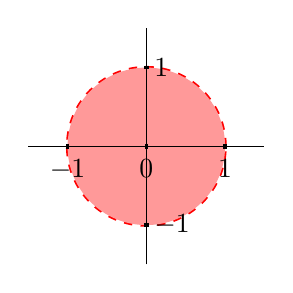
\begin{tikzpicture}
            \draw[red,very thick,dashed] (0,0) circle (1cm);
            \fill[red!40!white] (0,0) circle (1cm);
            \draw[step=.5cm,gray,very thin] (-1.4,1.4) grid (-1.4,1.4);
            \draw (-1.5,0) -- (1.5,0);
            \draw (0,-1.5) -- (0,1.5);
            \foreach \x in {-1,0,1}
                \draw[very thick] (\x cm, 1pt) -- (\x cm, -1pt) node[anchor=north] {$\x$};
            \foreach \y in {-1,1}
                \draw[very thick] (1pt, \y cm) -- (-1pt, \y cm) node[anchor=west] {$\y$};
        \end{tikzpicture}
    \end{center}
    Since $d_3((x_1,y_1),(x_2,y_2)) = |x_1-x_2|+|y_1-y_2|$, then if we set $(x_2,y_2) = (0,0)$, we get $d_3((x_1,y_1),(0,0)) = |x_1|+|y_1|$. Thus,
    $B_{d_3}(0,1) = \{(x,y): |x|+|y|<1\}$. From this, we can see that some of the boundary points of this set are the points $(0,1),(0,-1),(1,0),(-1,0)$ and
    $(0.5,0.5),(-0.5,-0.5),(-0.5,0.5),(0.5,-0.5)$. Extrapolating from these points, we can see that $B_{d_3}(0,1)$ is representated by the image:
    \begin{center}
        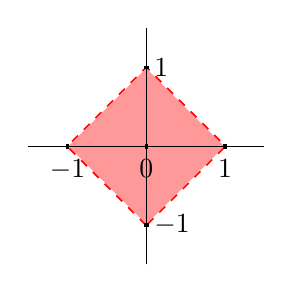
\begin{tikzpicture}
            \draw[red,very thick,dashed,shift={(0cm,0cm)},rotate=45] (-0.7,-0.7) rectangle (0.7,0.7);
            \fill[red!40!white,rotate=45] (-0.7,-0.7) rectangle (0.7,0.7);
            \draw[step=.5cm,gray,very thin] (-1.4,1.4) grid (-1.4,1.4);
            \draw (-1.5,0) -- (1.5,0);
            \draw (0,-1.5) -- (0,1.5);
            \foreach \x in {-1,0,1}
                \draw[very thick] (\x cm, 1pt) -- (\x cm, -1pt) node[anchor=north] {$\x$};
            \foreach \y in {-1,1}
                \draw[very thick] (1pt, \y cm) -- (-1pt, \y cm) node[anchor=west] {$\y$};
        \end{tikzpicture}
    \end{center}
    Observing the "rule" for $d_4$, we immediately see that $B_{d_4}(0,1) = \{(x,y):\:\text{max}\{|x|,|y|\}<1\}$. Thus, $B_{d_4}(0,1)$ contains
    any points contained by the lines $x=1,x=-1,y=1,y=-1$. This is given by the square as shown below:
    \begin{center}
        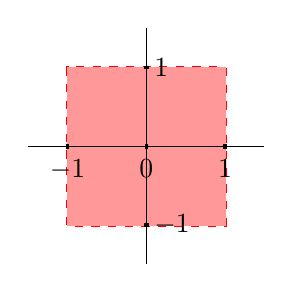
\begin{tikzpicture}
            \draw[red,very thick,dashed] (-1,-1) rectangle (1,1);
            \filldraw[red!40!white] (-1,-1) rectangle (1,1);
            \draw[step=.5cm,gray,very thin] (-1.4,1.4) grid (-1.4,1.4);
            \draw (-1.5,0) -- (1.5,0);
            \draw (0,-1.5) -- (0,1.5);
            \foreach \x in {-1,0,1}
                \draw[very thick] (\x cm, 1pt) -- (\x cm, -1pt) node[anchor=north] {$\x$};
            \foreach \y in {-1,1}
                \draw[very thick] (1pt, \y cm) -- (-1pt, \y cm) node[anchor=west] {$\y$};
        \end{tikzpicture}
    \end{center}

    \textbf{P3}.\\
    Let $X$ be a finite (cardinality) set equipped with a metric $d$. We show $d$ induces the discrete topology. Index $X$ so that $X = \{x_1,\hdots,x_k\}$ for
    some $k\in\mathbb{N}$. Then fix $x_i$ for some $1\leq i\leq k$ and let $\rho = $min$\{d(x_i,x_j): x_j\in X, x_j\neq x_i\}$. By property (ii) (defined in 
    \textbf{P1}) of a metric space, we know $\rho\neq 0$. Thus, choose $0<\xi<\rho$ for some $\xi\in\mathbb{R}$. Then, by construction of $\xi$, we 
    know that $B_{d}(x_i,\xi) = \{x_i\}$ so that $\{x_i\}$ is open in $\tau_{(X,d)}$. 
    Since $x_i$ is arbitrary, we can repeat this process again for some other $x_i$ to obtain that all singletons are open 
    in $\tau_{(X,d)}$ which implies that $\tau_{(X,d)}$ is the discrete topology (Lecture Exercises A1 \#4).\hfill$\blacksquare$\\

    \textbf{P4}.\\
    Let $f: X \to Y$ be a continouous function between topological spaces $X$ and $Y$ that are induced by the metrics $d$ and $d_Y$ respectively. We want to show
    $f_A: A \to Y$ is continouous if $A\subseteq X$ is a topological space metrized by the subspace metric $d_A$. Thus, choose $x,y\in A$ and $\epsilon > 0$. Then,
    note that since $d_A$ is the subspace metric of $A$, we have that $d_A(x,y) = d(x,y)$. Since $f$ is continuous, then we know that there exists a $\delta>0$ such
    that if $d(x,y)<\delta$ then $d_Y(f(x),f(y))<\epsilon$. Thus:
    \[ d_A(x,y) = d(x,y) < \delta \implies d_Y(f(x),f(y))<\epsilon \]
    By Theorem 21.1 (pg. 129), we have that this is enough to imply that $f_A$ is continuous.\hfill$\blacksquare$\\

    \newpage

    \textbf{P5}.\\
    Let $(X,\tau)$ be a topological space induced by a metric $d$ on $X$. Let $A\subseteq X$ be non-empty and define $\tau_A$ to be the subspace topology 
    on $A$. Furthermore, define the metric $d_A$ by the rule $d_A(x,y) = d(x,y)$ for all $x,y\in A$ (note it is straightforward to see that $d_A$ is a metric
    since $d$ is a metric and $A\subseteq X$) and define the topology $\tau_{d_A}$ to be the topology induced by the metric $d_A$ on $A$. We want to show that
    $\tau_{d_A} = \tau_A$.\\
    We know for a topology induced by a metric, the collection of all $\epsilon$-balls forms a basis for that space. Thus, define $\beta_X$ to be the collection
    of all $\epsilon$-balls given by the metric $d$, then $\beta_X$ is a basis for $\tau$. Furthermore, define $\beta = \{B' \cap A: B'\in\beta_X\}$. Since
    $\beta_X$ is a basis for $\tau$ and $\tau_A$ is a subspace topology of it, we obtain that $\beta$ is a basis for the subspace topology $\tau_A$. Similarly to before,
    define $\triangledown$ to be a basis for $\tau_{d_A}$ given by the collection of all $\epsilon$-balls given by the metric $d_A$. We claim these two bases 
    $\beta$ and $\triangledown$ are equivalent and prove it below.\\
    First, we show that for all $B\in\beta$, and for all $x\in B$, there exists $B'\in\triangledown$ such that $x\in B'\subseteq B$. Thus, choose an arbitrary
    $B\in\beta$ and from this, choose an arbitrary $x\in B$. From the definition of $\beta$, we can write $B$ as $H \cap A$ where $H$ is some $\epsilon$-ball in $X$.
    Suppose $H\subseteq A$. Then $B = H \cap A = H$ (note, this also implies $x\in H$). 
    Write $H = B_d(y,\epsilon)$ for some $\epsilon>0$, some $y\in X$ so that $d(x,y)<\epsilon$. Since $H\subseteq A$, it follows for any $x'\in H$, $x'\in A$ so that
    $d_A(y,x') =  d(y,x') < \epsilon$ which is enough to imply $B_d(y,\epsilon) = B_{d_A}(y,\epsilon)$ (the other containment direction follows similarly) so 
    that $H$ is an $\epsilon$-ball of $A$ and more specifically, $H\in\triangledown$.
    $H$ is an $\epsilon$-ball in $\beta_X$ and $\triangledown$. Thus, we have the existence of a set $H\in\triangledown$ such that $x\in H\subseteq H \cap A = B$ 
    as wanted. Now, suppose $H\subseteq A$ is not true. For any $\epsilon > 0$, we know $x\in B_{d_A}(x,\epsilon)\subseteq A$ (since $d_A$ is a metric on $A$).
    Also, since $H\in\tau$, we can find an $\epsilon$-ball around any point in $H$ such that the ball is contained in $H$ i.e. there exists $\epsilon_1>0$ such that
    $x\in B_d(x,\epsilon_1)\subseteq H$. So, now we have two $\epsilon$-balls centered at $x$. If $\epsilon_1 \leq \epsilon$, we get a similar case to if $H\subseteq A$,
    thus assume that $\epsilon_1 > \epsilon$. Since $B_{d_A}(x,\epsilon_1)\subseteq B_d(x,\epsilon_1)$ (by def'n of sub metric) $\subseteq H$, 
    it follows $B_{d_A}(x,\epsilon_1)\subseteq H$ and $B_{d_A}(x,\epsilon_1)\subseteq A$ so that $x\in B_{d_A}(x,\epsilon_1)
    \subseteq H \cap A = B$ as wanted. Since, we covered all cases (either $H\subseteq A$ or not), we are done for this direction.\\
    Now, we show that for all $B'\in\triangledown$, and for all $x\in B'$, there exists $B\in\beta$ such that $x\in B\subseteq B'$. Since $B'\in\triangledown$,
    we can write $B'$ as an $\epsilon$-ball i.e. $B' = B_{d_A}(y,\epsilon)$ for some $\epsilon>0$ and $y\in X$. Note, since $\epsilon > d_A(x,y) = d(x,y)$, we have
    that $x\in B_d(y,\epsilon)$. Note, $B_d(y,\epsilon) \cap A = \{x: d(x,y) < \epsilon\} \cap A = 
    \{ x\in A: d(x,y) < \epsilon\} = \{ x\in A: d_A(x,y) < \epsilon\} = B_{d_A}(y,\epsilon)$. Since $B_d(y,\epsilon)\cap A\in\beta$, it follows that:
    $x\in B_d(y,\epsilon) \cap A \subseteq B_{d_A}(y,\epsilon)$ as wanted.\\
    By Lemma 13.3, we have that the bases $\triangledown$ and $\beta$ are equivalent implying they generate the same topology. We have established that
    $\triangledown$ and $\beta$ generate $\tau_{d_A}$ and $\tau_A$ respectively. Thus, we must have that $\tau_A = \tau_{d_A}$ as wanted.\hfill$\blacksquare$\\

    \textbf{P6}.\\
    Let $X$ be a topological space equipped with the trivial topoloy. We show there is no metric $d$ that induces the topology $\tau$ on $X$. To do this, assume
    instead that one such metric exists and is called $d$. Since $d$ is a metric, then for all $x,y\in X$ such that $x\neq y$, we must have that
    $d(x,y)>0$. Also, since the collection of $\epsilon$-balls forms a basis for $\tau$, we must have that $B_d(x,\epsilon) = X$. To see why, suppose this was not
    true and instead $B_d(x,\epsilon) = A\subsetneq X$ ($A$ nonempty since $x$ is always in this set and $A$ a proper subset since $|X|>1)$, 
    since this is an $\epsilon$-ball, then this is an element of
    a basis on $\tau$ implying it is an open set in $X$ but this cannot be since $X$ is equipped with the trivial topology so only $X$ and $\emptyset$ are open.
    Thus $B_d(x,\epsilon)=X$ for all $\epsilon>0$ and $x\in X$. Fix $x_0\in X$. Suppose the set $A_{x_0} = \{x\in X, x\neq x_0: d(x,x_0)\}$ has a lower bound i.e.
    there exists $\delta>0$ such that the inequality $0 < \delta < d(x,x_0)$ holds for all $x\neq x_0$. Then consider the set $B_d(x_0,\delta)$. This contains
    $x_0$ since $d(x_0,x_0)=0$ (by metric map properties) but does not contain any other element of $X$ by our assumption of $\delta$ being a lower bound. Since
    $B_d(x_0,\delta)$ is a basis element but not an element of the indiscrete topology (singletons only open if $|X|=1$), we have a contradiction implying 
    that $d$ cannot be a metric if for some
    $x_0\in X$, the set $A_{x_0}$ has a lower bound. Now, instead assume that no such $x_0$ exists, i.e. there exists no $x_0\in X$ such that $A_{x_0}$ has a lower
    bound. This implies if the inequality $0<\delta<d(x,x_0)$ holds, there exists another $x'\neq x_0$ such that $d(x',x_0)<\delta$ which further implies that
    there exists $\epsilon_1>0$ and $\epsilon_2>0$ such that $B_d(x_0,\epsilon_1)\subsetneq B_d(x_0,\epsilon_2)$. Thus, we obtain the existence of a $y$ such that
    $y\in B_d(x_0,\epsilon_2)$ but $y\not\in B_d(x_0,\epsilon_1)$. However, this is a contradiction as we already established earlier that for all $\epsilon>0$, we
    have $B_d(x_0,\epsilon)=X$, more specifically, we should have that $B_d(x_0,\epsilon_1) = X = B_d(x_0,\epsilon_2)$ but we have just shown that there exists
    an element in $B_d(x_0,\epsilon_2)$ which doesnt exist in the other $\epsilon$-ball. Thus, we obtain a contradiction. Since, we have covered all cases,
    (either $d$ has a lower bound when compared to some element $x_0\in X$ or it does not), we obtain that a existence of a metric $d$ which induces the 
    indiscrete topology is impossible.\hfill$\blacksquare$\\

    \textbf{P7}.\\
    Assume $A\subseteq X$ is closed in $X$. We show that if $(x_n)$ is a convergent sequence (converging to $x\in X$) in $A$ (i.e. $(x_n)\subseteq A$), 
    then $x\in X$. We know that for any set $A\subseteq X$, $\overline{A} = A \cup \partial{A}$ (where $\partial{A}$ is the set of accumulation points of $A$).
    However, since $A$ is closed, we know that $\overline{A} = A$. Thus, $A = A \cup \partial{A}$ which is enough to imply that $\partial{A} \subseteq A$.
    It is left to show that $x$ is an accumulation point of $A$. By definition of an accumulation point, $x$ is an accumulation point of $A$ if and only if
    every open neighbourhood of $x$ contains at least one point of $A$ different from $x$. Since $(x_n)\to x$, we know that for all $\epsilon>0$, there exists a
    natural number $N > 0$ such that for all natural numbers $n > N$, $|x_n - x| < \epsilon$ ($X$ is metrizable, so we can use this definition). Additionally,
    since $X$ is metrizable, every neighbourhood is given by $B_d(x,\epsilon_1)$ where $d$ is the metric that induces the topology on $X$ and $\epsilon_1>0$ is arbitrary.
    Thus, it is left to show $B_d(x,\epsilon_1) - \{x\} \cap A \neq \emptyset$. Fix $\epsilon_1 > 0$. Then $(x_n)\to x$ tells us that there exists $n\in\mathbb{N}$
    such that $|x_n - x| < \epsilon$. Thus, $x_n \in B_d(x,\epsilon_1)$. This is enough to imply $B_d(x,\epsilon_1) - \{x\} \cap A \neq \emptyset$.\\
    
    Now, assume that every convergent sequence $(x_n)$ in $A$ converges to a point in $A$. We show that $A$ is closed. Using similar reasoning from the above paragraph,
    we know that if $(x_n)\to x$, then $x\in\partial{A}$. Since, we are given $x\in A$, this is enough to imply that $\partial{A}\subseteq A$. From this, we can
    obtain the result $A = A \cup \partial{A}$ and since we know $\overline{A} = A \cup \partial{A}$, then $A = \overline{A}$ which is enough to imply that $A$ is
    closed in $X$ as wanted.\hfill$\blacksquare$\\

    \textbf{P8}.\\
    We can see from the diagram below that in order to prove (a), (b) and (c) are equivalent, it suffices to show (1). (a) $\Leftrightarrow$ (b) and 
    (2). (b) $\Leftrightarrow$ (c).
    \begin{equation*}
        \begin{tikzcd}[column sep=small]
                         & (a) \arrow[dl, Leftrightarrow] & \\
            (b) \arrow[rr, Leftrightarrow] &              & (c)
        \end{tikzcd}
    \end{equation*}
    (1). Assume (a) holds. From page 137 of Munkres' Topology, we know that for every quotient map $p: X\to Y$, a subset $V$ of $Y$ is open in $Y$ if and only if
    $p^{-1}(V)$ is open in $X$. Since a set is defined to be open if and only if it is in the topology, we can rephrase this to: a subset $V\in\tau_Y$ if and only if 
    $p^{-1}(V)\in\tau_X$ which is enough to imply (b). Now, assume (b) holds. Since a set is defined to be open if and only if it is in the topology, we can rephrase
    (b) to mean: A subset $V\subseteq Y$ is open in $Y$ if and only if the subset $p^{-1}(V)\subseteq X$ is open in $X$. Since, we are given a global assumption
    that $p$ is surjective, these two conditions are enough to imply that (a) holds (def'n of quotient map).\\
    (2). Assume (b) holds. Let $V$ be an open set of $Y$. By (b), we know that $p^{-1}(V)$ is open. Note, since $p^{-1}(V^c) = (p^{-1}(V))^c$, we have that,
    since $V^c$ is closed ($V$ open), then $p^{-1}(V^c) = [p^{-1}(V)]^c$ is closed (since it is the complement of an open set). Now, let $[p^{-1}(V)]^c$ be some
    closed set in $X$, this implies $p^{-1}(V)$ is open so that $p^{-1}(V)\in\tau_X$. By (b), we know that this implies $V\in\tau_Y$ which implies $V$ is open in
    $Y$ which implies $V^c$ is closed in $Y$. Thus $p^{-1}(V)^c$ closed in $X$ implies $V$ closed in $Y$. Therefore $p^{-1}(V)^c$ is closed in $X$ if and only if
    $V^c$ is closed in $Y$. This is enough to imply (c). Now, instead, suppose (c) holds. Choose $C$ closed in $Y$ (so that $V := C^c$ is open), then 
    consider $p^{-1}(V) = p^{-1}(C^c) = p^{-1}(C)^c$ which is clearly open in $X$. Thus, $V$ open in $Y \implies p^{-1}(V)$ is open in $X$ or equivalently,
    $V\in\tau_Y \implies p^{-1}(V)\in\tau_X$.  Now, choose
    $p^{-1}(C)$ closed in $X$ (so that $p^{-1}(V) := p^{-1}(C)^c$ is open). By (c), we have that $C$ is closed in $Y$ which implies $C^c$ is open in $Y$. Thus,
    $p^{-1}(C)^c = p^{-1}(C^c) = p^{-1}(V)\in\tau_X \implies V\in\tau_Y$. Therefore, we obtain that $p^{-1}(V)\in\tau_X$ if and only if $V\in\tau_Y$ which is enough
    to imply (b). Therefore (1) and (2) holds as wanted and our diagram is completely proven implying (a), (b) and (c) are equivalent.\hfill$\blacksquare$\\

    \textbf{P9}.\\
    Let $f: X\to Y$ be a bijective continuous map between topological spaces. Assume $f$ is a quotient map. Since $f$ is already bijective and continuous, to show
    $f$ is a homeomorphism, we have to show the inverse $f^{-1}$ (whose existence is given by the bijective assumption) is also continuous. Note, $f^{-1}$ is
    a mapping from $Y\to X$, so to show it is continuous, we have to show a set $V$ in $X$ is open if and only if $f(V)$ is open in $Y$ i.e. a set is open in $X$
    if and only if the pre-image of the inverse (which is just the image of $f$) of the set is open in $Y$. From the definition of a quotient map, we know that
    $f$ is open, therefore the map $f^{-1}$ fulfills this condition, thus we obtain that $f^{-1}$ is continuous so that $f$ is a homeomorphism.\\
    Let $g: X\to Y$ be a bijective continuous map between topological spaces. Assume $g$ is a homeomorphism, we show $g$ is a quotient map. Since $g$ is a homeomorphism,
    we know that $g$ is bijective so that in particular, $g$ is surjective which is a required condition for $g$ to be a quotient map. It remains to be proven that
    every subset $V$ of $Y$ is open if and only if $g^{-1}(V)$ is open in $X$. So, assume a subset $V$ of $Y$ is open. By the continuity of $g$, it is clear that
    $g^{-1}(V)$ is open in $X$ (def'n of continuity). Now, assume $g^{-1}(V)$ is open in $X$. In class, we stated that all homeomorphisms are open maps, therefore,
    it follows that if $g^{-1}(V)$ is open in $X$, then $g(g^{-1}(V)) = V$ (equality follows due to surjectivity) is open in $Y$. Therefore, $g$ is a quotient map.\hfill
    $\blacksquare$.\\

    \textbf{P10}.\\
    (a): A figure 8 composed of two circles intersecting at a point:
    \begin{equation*}
    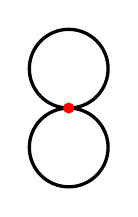
\begin{tikzpicture}
        \draw[very thick] (3,0.5) circle [radius=0.5];
        \draw[very thick] (3,1.5) circle [radius=0.5];
        \fill[red] (3,1) circle[radius=2pt];
    \end{tikzpicture}
    \end{equation*}
    (b): We obtain $D^2/S^1 \cong S^2$ so that one homeomorphic image of the quotient image looks like:
    \begin{equation*}
        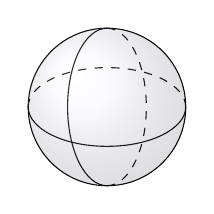
\begin{tikzpicture}
                \draw (-1,0) arc (180:360:1cm and 0.5cm);
                \draw[dashed] (-1,0) arc (180:0:1cm and 0.5cm);
                \draw (0,1) arc (90:270:0.5cm and 1cm);
                \draw[dashed] (0,1) arc (90:-90:0.5cm and 1cm);
                \draw (0,0) circle (1cm);
                \shade[ball color=blue!10!white,opacity=0.20] (0,0) circle (1cm);
        \end{tikzpicture}
    \end{equation*}

\end{document}
